\documentclass[9pt]{beamer}
\usetheme[titlepagelogo=minerva2,% Logo for the first page
						language=italian
                        ]{TorinoTh}
                        
\usepackage[beamer,customcolors]{hf-tikz}
\usepackage{verbatim}
\usepackage{algorithm}
\usepackage{longtable}
\usepackage{subcaption}
\usepackage[noend]{algpseudocode}
\hfsetfillcolor{alerted text.fg!10}
\hfsetbordercolor{alerted text.fg}

\author{Marco Odore}
\rel{Prof. Giorgio Valentini}
\assistantsupervisor{Dr. Marco Notaro}
\title[Metodi di Ensemble Gerarchici]{Metodi di Ensemble Gerarchici per la Predizione Strutturata della Funzione delle Proteine}
\ateneo{Università Degli Studi Di Milano}
\date{10 Luglio 2018}

\begin{document}
\titlepageframe
\begin{tframe}{Il problema della predizione della funzione delle proteine}
  % 
  \begin{columns}
    %
    \begin{column}{.65\textwidth}
      \minipage[c][0.4\textheight][s]{\columnwidth}
	   \begin{itemize}	
      \onslide<1->
	  \item Identificare la funzione delle proteine attraverso le analisi di laboratorio è \highlightbf{costosa} e richiede \highlightbf{molto tempo}
	  \onslide<2->
	  \item Esistono migliaia di funzioni a cui poter associare un gene/proteina, anche contemporaneamente \highlightbf{(problema multiclasse e multietichetta)}
      \onslide<3->
	  \item Il quantitativo di dati genomici cresce molto rapidamente.
      \onslide<4->
      \item Le classi che rappresentano le diverse funzioni delle proteine \highlightbf{non sono indipendenti}.
	  \onslide<5->
	  \item La \highlightbf{classificazione manuale} delle proteine è quindi infattibile. È necessario quindi un approccio \highlightbf{automatico}.
	  \end{itemize}
      \endminipage      
    \end{column}
    %
    \begin{column}{.35\textwidth}
      % for top aligned images use minipage
      \only<1-5>{
        \minipage[c][0.4\textheight][s]{\columnwidth}
        \onslide<1->    
        \only<1-5>{
          \begin{figure}
            \centering
            \includegraphics<1>[scale=0.15]{img/lab3.jpg} %         
            \includegraphics<2>[scale=0.3]{img/multilabel.png}%
            \includegraphics<3>[scale=0.16]{img/growth.jpg}
            \includegraphics<4>[scale=0.3]{img/relation.png}
            \includegraphics<5>[scale=0.1]{img/machinelearning.png}
        \end{figure}}
       \endminipage
      }   
      % for vertically centered images use parbox
    \end{column}
  \end{columns}
\end{tframe}

\begin{tframe}{Tassonomie per le funzioni delle proteine}
\begin{itemize}
\onslide<1->
\item Esistono due tassonomie principali per l'organizzazione delle funzioni:
\begin{itemize}

\onslide<2->
\item \highlightbf{Gene Ontology} (GO): organizza le funzioni come un grafo diretto aciclico (DAG), ed è articolata in tre ontologie differenti: \highlight{Biological Process} (BP), \highlight{Molecular Function} (MF) e \highlight{Cellular Component} (CC). 
\onslide<3->
\item \highlightbf{Functional Catalogue} (FunCat): è organizzato invece come un albero, e descrive le funzioni in maniera più sintetica rispetto alla Gene Ontology.
\end{itemize}
\onslide<4->
\begin{figure}[h]
\center
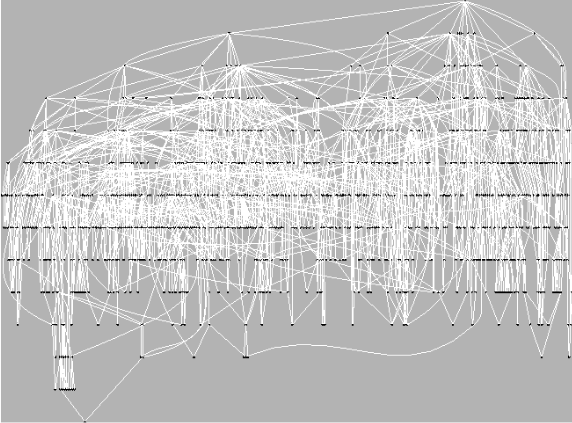
\includegraphics[scale=0.15]{./img/GO.png}
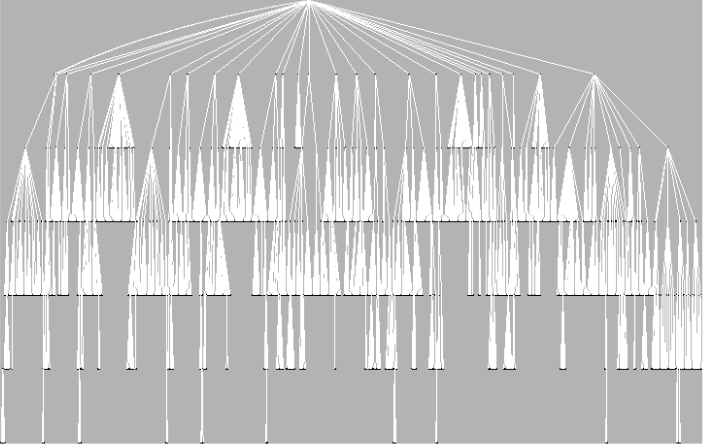
\includegraphics[scale=0.14]{./img/FunCat.png}
\label{DAGTREE}
\end{figure}
\onslide<5->
\item Data la granularità e specificità superiori della GO e il suo largo utilizzo nella comunità scientifica, nella tesi si è utilizzata tale ontologia.
\end{itemize}  
\end{tframe}

\begin{tframe}{La predizione della funzione delle proteine tramite metodi automatici}
Schematicamente i metodi per effettuare predizioni della funzione delle proteine in maniera automatica si possono classificare in [\emph{Valentini, 2014}]:

\begin{itemize}
\onslide<2->
\item Metodi basati sulla \highlightbf{comparazione di biosequenze}: si basano sull'idea che sequenze simili condividano funzioni simili.
\onslide<3->
\item Metodi \highlightbf{basati su reti}: sono metodi applicati a dati rappresentati sotto forma di reti, che si basano sugli algoritmi di propagazione delle etichette.
\onslide<4->
\item Metodi \highlightbf{flat supervisionati} (es. basati su metodi di apprendimento supervisionato).
\onslide<5->
\item Metodi \highlightbf{Kernel per spazi di output strutturato}: sono metodi che sfruttano funzioni kernel congiunte per predire in spazi di output strutturato.
\onslide<6->
\item Metodi \highlightbf{Ensemble Gerarchici}: i metodi trattati in questa tesi.
\end{itemize}

\end{tframe}

\begin{tframe}{Metodi Ensemble Gerarchici 1/2}
I Metodi di Ensemble Gerarchici sono metodi caratterizzati da due step principali [\emph{Valentini, 2014}]:

\begin{enumerate}
\onslide<2->
\item \highlightbf{Predizione flat} delle diverse classi dell’ontologia, generando diversi predittori \emph{indipendenti}.
\onslide<3->
\item \highlightbf{Combinazione e correzione gerarchica delle predizioni} sfruttando il DAG dei termini della GO.
\end{enumerate}
\onslide<4->
Il secondo step rappresenta la componente \emph{ensemble} del metodo. Tale step si rende necessario in quanto le predizioni flat non tengono in considerazione la struttura gerarchica dei DAG della GO, portando a risultati \emph{inconsistenti}.
\onslide<5->
\block{Consistenza \& True Path Rule}
Un insieme di predizioni $\hat{y} = <\hat{y}_1, \hat{y}_2, \dots, \hat{y}_{|N|}>$, dove $|N|$ è la cardinalità dei termini della gerarchia, è definito \emph{consistente}, se rispetta la \emph{True Path Rule}, e cioè:
\[
y\;\;\;consistente\;\; \leftrightarrow \forall i \in N, j \in par(i) \rightarrow y_j \geq y_i
\] 
Dove $par(i)$ indica l'insieme dei termini genitori del nodo $i$ nella gerarchia.
\endblock{}
\end{tframe}

\begin{tframe}{Metodi Ensemble Gerarchici (Esempio) 2/2}
\begin{center}
\includegraphics<1>[width=5cm]{img/1_1.png}
\includegraphics<2>[width=5cm]{img/2.png}
\includegraphics<3>[width=5cm]{img/3.png}
\includegraphics<4>[width=8.22cm]{img/4.png}
\end{center}

\end{tframe} 


\begin{tframe}{Metodi Ensemble Gerarchici: Approcci}
\begin{columns}
    \begin{column}{.50\textwidth}
      \minipage[c][0.4\textheight][s]{\columnwidth}
      Esistono fondamentalmente due approcci generali per la correzione [\emph{Valentini, 2011}]:
	   \begin{itemize}
	   \onslide<2->
	  \item \highlight{Top-down}: le predizioni vengono corrette dai nodi più generali a quelli più specifici.
	   \onslide<3->	  
	  \item \highlight{Bottom-up}: Le predizioni vengono corrette dai nodi più specifici verso quelli più generali.
      \end{itemize}
      \endminipage 
    \end{column}
    %
    \begin{column}{.50\textwidth}
    \onslide<2-> 
        \minipage[c][0.4\textheight][s]{\columnwidth}
        \only<2-3>{
          \begin{figure}
            \centering
            \includegraphics<2>[scale=0.3]{img/topdown.png}
            \includegraphics<3>[scale=0.3]{img/bottomup.png}
        \end{figure}}
        \endminipage
    \end{column}
  \end{columns}
\end{tframe}

\begin{tframe}{Metodo Top-Down Gerarchico (HTD-DAG)}
\begin{itemize}

\onslide<1->
\item È un metodo che utilizza l'approccio \emph{Top-Down} [\emph{Notaro et al., 2017}].
\onslide<2->
\item La correzione avviene ricorsivamente, percorrendo il grafo per \emph{livelli}\footnote{\footnotesize{Dove il livello è quello del cammino massimo dalla radice}}. Più precisamente, dato il grafo $G = (N, E)$, gli score flat $f(x) = \hat{y}$ sono corretti gerarchicamente a $\bar{y}$, applicando la seguente regola:
\begin{block}{Aggiornamento con HTD-DAG}
\[
\bar{y}_i := 
\begin{cases}
\hat{y}_i \;\;\;\;\;\;\;\;\;\;\;\;\;\;\;\;\;\;\;\;\; if\;\; i \in root(G)\\
min_{j \in par(i)} \bar{y}_j \;\;\;\; if \;\; min_{j \in par(i)}\bar{y}_j < \hat{y}_i\\
\hat{y}_i \;\;\;\;\;\;\;\;\;\;\;\;\;\;\;\;\;\;\;\;\; altrimenti
\end{cases}
\]
\end{block}
Dove $par(i)$ specifica i genitori del nodo $i$.
\end{itemize} 
\end{tframe}

\begin{tframe}{Metodo True Path Rule per DAG (TPR-DAG)}
\begin{itemize}
\onslide<1->
\item È un metodo che combina gli approcci top-down e bottom-up per la correzione delle predizioni flat ([\emph{Valentini, 2011}], [\emph{Cesa Bianchi et al., 2012}] per ontologie ad albero, [\emph{Notaro et al., 2017}] per DAG). 
\onslide<2->
\item È suddiviso in due step sequenziali:
\begin{enumerate}
\onslide<3->
\item \highlightbf{Step bottom-up}: che partendo dai nodi più specifici del DAG, propaga quelle predizioni flat che sono considerate \highlight{positive}.
\onslide<4->
\item \highlightbf{Step top-down}: È il medesimo step utilizzato dal metodo HTD-DAG.
\end{enumerate}
\onslide<5->
\item Lo step top down si rende necessario in quanto la propagazione delle predizioni positive dal basso verso l’alto non garantisce la consistenza delle predizioni necessarie alla True Path Rule. 
\onslide<6->
\item La selezione dei nodi considerati \emph{positivi} può avvenire in diverse maniere: con \highlight{soglia adattiva}, \highlight{senza soglia} e con \highlight{soglia fissa}.
\end{itemize}
\end{tframe}

\begin{tframe}{Generalized Pool Adjacent Violator (GPAV) (1/5)}
\begin{itemize}
\onslide<1->
\item Per il passo Top-Down dell’algoritmo TPR-DAG (e HTD) è stato sviluppato un nuovo metodo all'interno di questa tesi, e cioè \highlightbf{Generalized Pool Adjacent Violator} (GPAV) [\emph{Burdakov et al., 2006}], un algoritmo che permette di risolvere i problemi di \highlightbf{Isotonic Regression}, definiti come:
\begin{block}{Isotonic Regression (caso generale con ordinamento parziale)}
Dato un DAG, $G(N, E)$, con il set di nodi $N = \{1, 2, ..., n\}$, si deve trovare il vettore $x^{*}\in R^{n}$ tale che:
\[
min \sum_{i=1}^{n} w_i (x_i - a_i)^2
\]
\begin{center}
such that $x_i \le x_j$ $\forall (i,j) \in E $ 
\end{center}
\end{block} 
\onslide<2->
\item Con una complessità pari a $O(n^2)$.
\end{itemize}
\end{tframe}


\begin{tframe}{Generalized Pool Adjacent Violator (GPAV) (2/5)}
Esempio di Isotonic Regression con \emph{ordinamento totale}:
\begin{figure}
\centering
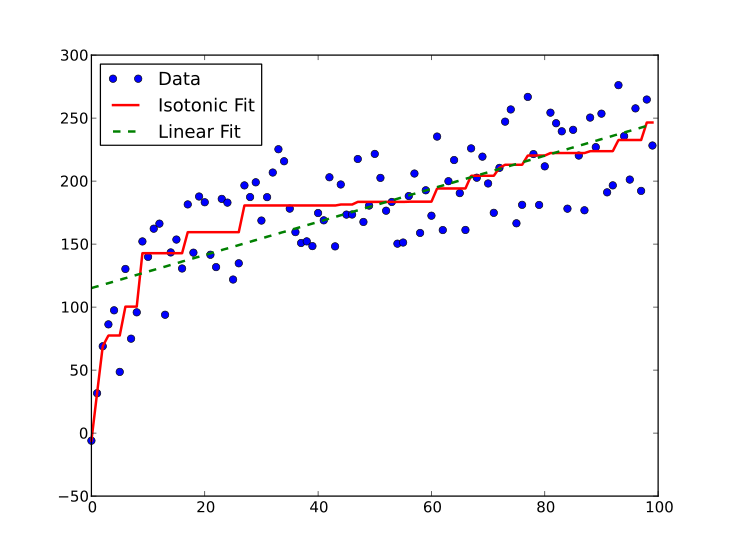
\includegraphics[scale=0.3]{img/monotonic.png}
\end{figure}
\end{tframe}
\begin{tframe}{Generalized Pool Adjacent Violator (GPAV) (3/5)}
\begin{itemize}
\onslide<1->
\item L'algoritmo richiede un \highlight{ordinamento topologico} del grafo.
\onslide<2->
\item L’algoritmo genera uno split del set di nodi $N$ del DAG, in un insieme di \highlight{blocchi disgiunti} (inizialmente il numero di blocchi è uguale a $|N|$).
\onslide<3->
\item Seguendo l'ordinamento topologico del grafo, un blocco \highlight{assorbe} un suo blocco \emph{predecessore} se si verificano determinate condizioni.
\onslide<4->
\item I nodi presenti nel medesimo blocco $B_i$ \highlight{condividono il medesimo valore} $x_i$, e quindi a seguito dell'assorbimento sarà necessario un aggiornamento di tale valore.
\end{itemize}
\end{tframe}

\begin{tframe}{Generalized Pool Adjacent Violator (GPAV e ISO-TPR) (4/5)}
\onslide<1->
\begin{center}
\scalebox{0.6}{
    \begin{minipage}{0.90\linewidth}
\begin{algorithm}[H]
\caption{GPAV}\label{gpav}
\begin{algorithmic}[1]
\State \textbf{Input: }
\State $G = (N, E)$
\State $N = \{1, 2, ..., |N|\} $ 
\State $\hat{y} = <\hat{y}_1, \hat{y}_2, ...,\hat{y}_{|N|}>$
\Procedure{GPAV}{}
\For{(each $i \in N$)}
\State $B_i = \{i\}$ 
\State $B_i^{-} = i^{-}$
\State $x_i = \hat{y}_i$
\State $W_i = w_i$
\EndFor
\For{$k = 1, 2, ..., n$}
\State \emph{// finché esiste un predecessore di $B_{k}$ che viola la monotonicità}
\While{$\{i \in B_k^{-}: x_i > x_k\}\neq 0$} 
\State \emph{// Trova l'elemento che viola maggiormente il vincolo}
\State \textbf{Find} $j \in B_k^{-}: x_j = max\{x_i : i \in B_k^{-}\}$ 
\State \textbf{Absorb(k, j)} \emph{// $j$ viene assorbito da $B_k$}
\EndWhile
\EndFor
\State \emph{//Aggiornamento per soluzione finale }  
\For{each $k \in H$}
\For{each $i \in B_k$}
\State $\bar{y}_i = x_i$  
\EndFor
\EndFor
\EndProcedure
\State \textbf{Output: }
\State $\bar{y} = <\bar{y}_1, \bar{y}_2, ...,\bar{y}_{|N|}>$
\end{algorithmic}
\end{algorithm}
\end{minipage}}
\end{center}
\end{tframe}
\begin{tframe}{Generalized Pool Adjacent Violator (GPAV e ISO-TPR) (5/5)}
\begin{itemize}
\onslide<1->
\item Riassumendo, l’algoritmo effettua degli assorbimenti di blocchi adiacenti, finché questi violano i vincoli del problema quadratico, generando di fatto una partizione dei nodi, in cui le parti condividono lo stesso valore.
\onslide<2->
\item Sostituendo GPAV allo step Top-Down dell'algoritmo TPR-DAG visto in precedenza (invece che HTD), si ottiene l'algoritmo \highlightbf{ISO-TPR}, un altro nuovo metodo utilizzato in questa tesi.
\onslide<3->
\item Il passo bottom-up di TPR permette di aumentare la sensibilità (Recall) e l'algoritmo GPAV nello step top-down assicura la consistenza, manetenendo gli score il più vicino possibile agli score ottenuti nel passo bottom-up (nel senso dei minimi quadrati).
\end{itemize}
\end{tframe}

\begin{tframe}{Predizione della funzione delle proteine in C.elegans (WORM)}
\begin{itemize}
\onslide<1->
\item Si è eseguita la sperimentazione sul genoma della specie
\highlight{Caenorhabditis elegans} (WORM), utilizzando come insieme delle  istanze e input del problema una matrice simmetrica generata dal network di interazione proteina-proteina \highlight{STRING} [\emph{Szklarczyk et al., 2015}] \footnote{\footnotesize{Search Tool for the Retrieval of Interacting Genes/Proteins}}.
\onslide<2->
\item Tale matrice STRING ha dimensione 15752×15752 (WORM). Il nostro problema ha quindi 15752 istanze.
\onslide<3->
\item In base al tipo di ontologia, si hanno DAG con un quantitativo diverso di nodi(termini) e archi(relazioni): 

\begin{table}[h]
\centering
\resizebox{.5\textwidth}{!}{
\begin{tabular}{|l|l|l|}
\hline
      \textbf{ ontologia} & \textbf{numero di termini} & \textbf{numero di archi} \\ \hline
BP & 4068  &  8066   \\ 
\hline
MF  & 1163  & 1567   \\ 
\hline
CC  & 578  & 1082     \\ 
\hline
\end{tabular}}

\label{DAG_desc}
\end{table}
\end{itemize}
\end{tframe}

\begin{tframe}{Annotazioni per il dataset C.elegans (WORM)}
Per evitare di avere problemi nella fase di cross-validazione, i DAG sono stati ridotti a quei termini per cui si hanno almeno 10 annotazioni. Un po' di statistiche a seguito della selezione:
\begin{table}[h]
\centering
\begin{tabular}{|l|l|l|l|l|l|}
\hline
\textbf{Onto} & \textbf{numero di termini} & \textbf{media} & \textbf{d.std.} & \textbf{massimo} & \textbf{minimo} \\ \hline
BP            & 1335                & 71,33                & 151,68              & 2597                & 10                  \\ \hline
MF            & 186                 & 61,23                & 191,84              & 1806                & 10                  \\ \hline
CC            & 221                 & 131,9                & 302,25              & 1924                & 10                  \\ \hline
\end{tabular}
\caption{\footnotesize{La colonna \emph{numero di termini} indica il numero di termini ottenuti dopo la selezione, \emph{media} la media delle annotazioni per classe, per l'ontologia di riferimento, \emph{d.std.} la deviazione standard delle annotazioni per l'ontologia di riferimento, \emph{massimo} e \emph{minimo} rispettivamente il massimo e minimo numero di annotazioni.}}
\label{riduzioneann}
\end{table}
\end{tframe}

\begin{tframe}{Algoritmi di ML per le predizioni flat}
\begin{itemize}
\onslide<1->
\item Per quanto riguarda gli algoritmi di apprendmento automatico da utilizzare per le predizioni flat, si sono considerati i seguenti metodi:
\begin{enumerate}
\footnotesize{
\item \emph{K-Nearest Neighbors}
\item \emph{Logit Boost}
\item \emph{Linear Discriminant Analysis}
\item \emph{eXtreme Gradient Boosting} 
\item \emph{C5.0} (Alberi di decisione)
\item \emph{Random Forest}
\item \emph{Multilayer Perceptron}
\item \emph{Support Vector Machine lineare}
\item \emph{Bagged CART} (Bagged ensemble di alberi di decisione)
\item \emph{AdaBoost.M1}
\item \emph{Naive Bayes}
\item \emph{Modelli Lineari Generalizzati}}
\end{enumerate}
\onslide<2->
\item Dato l'elevato numero di algoritmi selezionati per la sperimentazione, si è deciso di \highlight{non effettuare il tuning dei parametri}, questo per evitare di allungare ulteriorimente i tempi dell'intero processo di valutazione e generazione degli score flat.
\end{itemize}
\end{tframe}

\begin{tframe}{Cross-validazione e metriche usate per la valutazione degli algoritmi}
\begin{columns}

    \begin{column}{.65\textwidth}
      \minipage[c][0.4\textheight][s]{\columnwidth}
	   \begin{itemize}	
      		\onslide<1->
	  		\item Per stimare le performance dei nostri predittori si è utilizzata la tecnica della \highlight{cross-validazione}. 
	  		\onslide<2->
	  		\item Come metriche si sono poi usate la:
	  		\begin{enumerate}
	  			\onslide<3->
				\item \highlight{AUROC}: mette in relazione le misure di Recall e False Positive Rate, al variare di una soglia applicata all’output del modello.
				\onslide<4->	  			
				\item \highlight{AUPRC}: è una misura che mette in relazione la variazione di Precision al variare della Recall. 
				\onslide<5->
	  			\item \highlight{F-Score gerarchica}: è una metrica centrata sui geni, massimizzata al variare di una soglia t in (0, 1). Tale misura si basa sulla Precisione e Recall centrate sui geni e non su le classi.
	  		\end{enumerate}
	  \end{itemize}
      \endminipage      
    \end{column}
    
    
    \begin{column}{.35\textwidth}
      % for top aligned images use minipage
      \only<1-5>{
        \minipage[c][0.4\textheight][s]{\columnwidth}
        \onslide<1->    
        \only<1-5>{
          \begin{figure}
            \centering
            \includegraphics<1>[scale=0.16]{img/cross10fold.png} %         
            \includegraphics<3>[scale=0.14]{img/AUROC.png}%
            \includegraphics<4>[scale=0.34]{img/AUPRC.png}
            \includegraphics<5>[scale=0.27]{img/Fscore.png}
        \end{figure}}
       \endminipage
      }   
      % for vertically centered images use parbox
    \end{column}


\end{columns} 
\end{tframe}

\begin{tframe}{Stima preliminare dei tempi di calcolo degli algoritmi flat}

\begin{center}
Cross-validation 10 fold - No tuning - Campione 10 classi
\end{center}
\begin{figure}[hp!]
\center
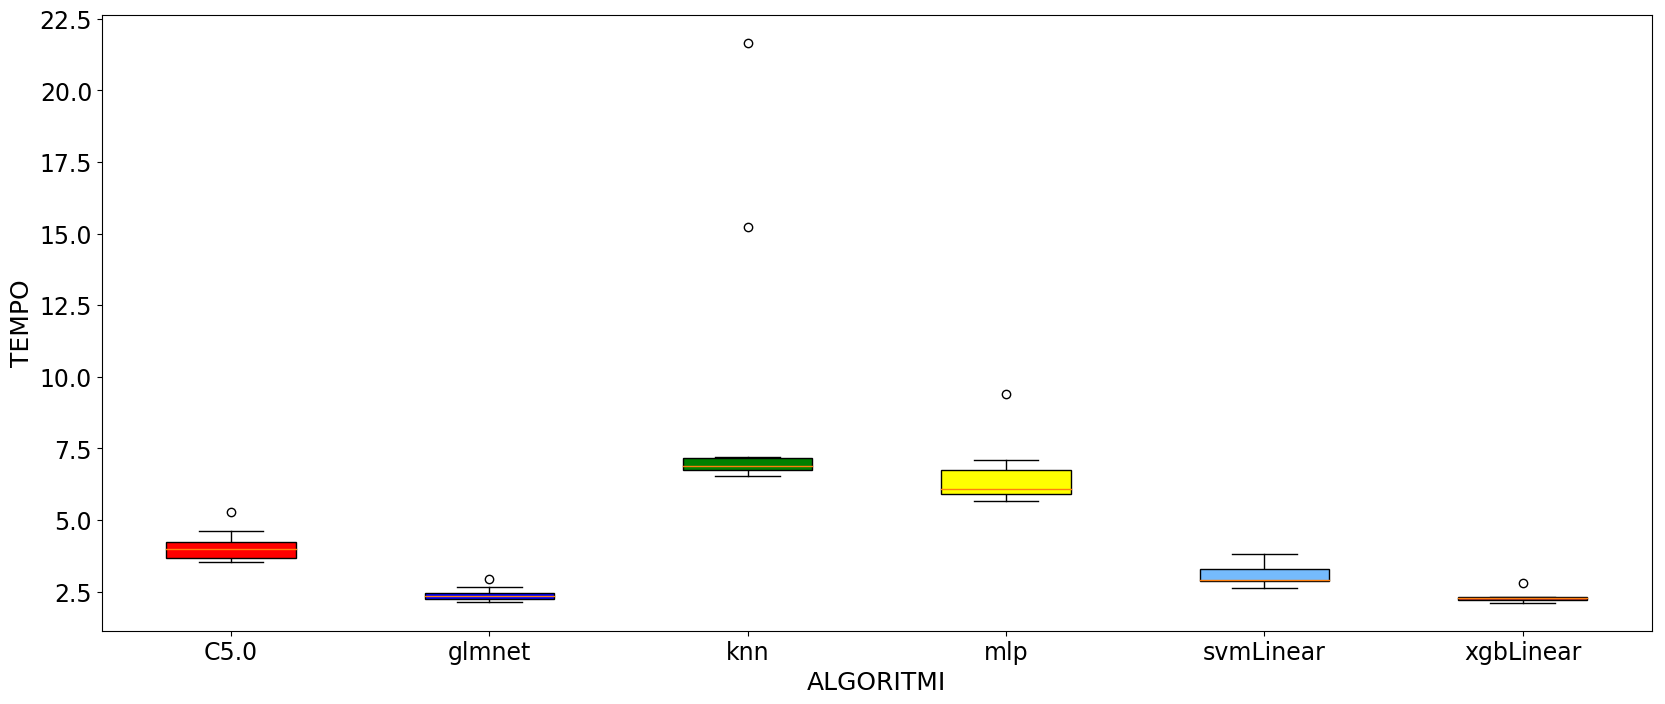
\includegraphics[scale=0.25]{../images/BP_box_plot_times.png}

\caption{\footnotesize{Il box plot dei tempi di esecuzione, con cross-validation a 10 fold per l' ontologia BP. I tempi sono da intendersi in ore e per classe, per un campione di 10 classi.}}
\label{boxplot_p}
\end{figure}
\end{tframe}

\begin{tframe}{Riduzione dei tempi di calcolo del problema}

\begin{columns}
    \begin{column}{.60\textwidth}
      \minipage[c][0.4\textheight][s]{\columnwidth}
		\begin{itemize}
			\onslide<1->
				\item Si è prima di tutto ridotto il numero di fold da 10 a 5 nella cross-validation
			\onslide<2->
				\item Si sono provati due metodi di riduzione della dimensionalità:
				\begin{enumerate}
				\onslide<3->
					\item \highlightbf{Selezione delle feature con Correlazione di Pearson} (FS).
				\onslide<4->
					\item \highlightbf{Selezione delle componenti con la Principal Component Analysis} (PCA)
				\end{enumerate}
		\onslide<5->
		\item Sempre facendo una stima sul medesimo campione di 10 classi, si sono testate:
		\begin{enumerate}
		\item configurazioni per la FS per le prime 1000, 500 e 100 feature nel ranking ottenuto (a destra BoxPlot per le prime 100 feature selezionate) 
		\onslide<6->
		\item configurazioni per la PCA, per le componenti che selezionano rispettivamente il 90\%, il 70\% e il 50\% della varianza spiegata (a destra BoxPlot per le prime 15 componenti = 50\% varianza spiegata)
		\end{enumerate}
		\end{itemize}	
	 \endminipage
	\end{column}
	
	\begin{column}{.40\textwidth}
      % for top aligned images use minipage
      \only<1-6>{
        \minipage[c][0.4\textheight][s]{\columnwidth}
        \onslide<1->    
        \only<1-6>{
          \begin{figure}
            \centering
            \includegraphics<1>[scale=0.26]{img/cross_val.png} %         
            \includegraphics<3>[scale=0.3]{img/Pearson.png}%
            \includegraphics<4>[scale=0.18]{img/PCA.png}
            \includegraphics<5>[scale=0.12]{../images/FS_BP_times.png}
            \includegraphics<5>[scale=0.12]{../images/FS_BP_auroc.png}
            \includegraphics<5>[scale=0.12]{../images/FS_BP_auprc.png}
            \includegraphics<6>[scale=0.12]{../images/PCA_BP_times.png}
            \includegraphics<6>[scale=0.12]{../images/PCA_BP_auroc.png}
            \includegraphics<6>[scale=0.12]{../images/PCA_BP_auprc.png}
        \end{figure}}
       \endminipage
      }  
      \end{column} 
\end{columns}
\end{tframe}

\begin{tframe}{Organizzazione degli esperimenti}
\onslide<1->
Data l'analisi precedente effettuata sugli algoritmi di apprendimento flat (su di un campione di 10 classi), si è deciso di adottare il seguente set-up sperimentale: 

\begin{itemize}
\item \highlightbf{cross-validation 5 fold + Selezione delle prime 100 feature con Correlazione di Pearson}.
\item \highlightbf{cross-validation 5 fold + Selezione delle prime 15 componenti della PCA}.
\end{itemize} 
Le quali hanno evidenziato un buon compromesso tra tempi di esecuzione e performance.  
\newline
\newline
\onslide<2->
Per quanto riguarda i metodi ensemble gerarchici, si sono utilizzati i seguenti metodi:

\begin{enumerate}
\item \highlightbf{HTD-DAG} [\emph{Notaro et al., 2017}]
\item \highlightbf{TPR-DAG} (con variante senza soglia, con soglia adattiva, con pesi nell'aggiornamento) [\emph{Notaro et al., 2017}]
\item \highlightbf{GPAV} (nuovo metodo introdotto in questa tesi)
\item \highlightbf{ISO-TPR} (nuovo metodo introdotto in questa tesi, con variante senza soglia e con soglia adattiva)
\end{enumerate}

\end{tframe}

\begin{tframe}{Performance degli algoritmi flat con FS e PCA}
La generazione di tutti gli score flat, per entrambi i metodi di riduzione della complessità, ha evidenziato delle performance generalmente migliori per la selezione delle feature effettuta con la correlazione di Pearson (Test dei ranghi con segno di Wilcoxon, con significatività $\alpha = 0.01$). Le performance migliori sono probabilmente da ricondurre al fatto che il tipo di riduzione per la correlazione è \emph{supervisionato} a differenza della PCA.

\begin{figure}[h!]
\centering
\hspace*{-0.3in}
\includegraphics<2>[scale=0.28]{../images/FS_vs_PCA_BP_AUROC.png}
\includegraphics<3>[scale=0.28]{../images/FS_vs_PCA_BP_AUPRC.png}
\end{figure}

\end{tframe}

\begin{tframe}{Risultati Metodi Ensemble}
I metodi ensemble risultano essere più efficaci e riescono a migliorare in maniera statisticamente significativa i metodi flat (Test dei ranghi con segno di Wilcoxon, con significatività $\alpha = 0.01$) quando è utilizzata la selezione delle feature con correlazione di Pearson come tecnica di riduzione della dimensionalità. (HTD è un'eccezione)

\only<2>{
\begin{table}[h!]
\caption*{\textbf{\highlightbf{Confronto fra metodi gerarchici e metodi flat (AUROC).}}}

                    \resizebox{.3\textwidth}{!}{
                    \begin{subtable}[t]{0.4\textwidth}
                    \centering\footnotesize
\caption{ \textbf{[AUROC] [BP] [FS]}}
\begin{tabular}{|l|l|}
\hline
 \textbf{METODI GERARCHICI} & \textbf{WIN-TIE-LOSS} \\ \hline
 \textbf{GPAV} &12-0-0\\ \hline
 \textbf{HTD} &1-4-7\\ \hline
 \textbf{TPR-TF} &11-1-0\\ \hline
 \textbf{ISO-TPR-TF} &12-0-0\\ \hline
 \textbf{TPR-AT} &5-1-6\\ \hline
 \textbf{ISO-TPR-AT} &11-1-0\\ \hline
 \textbf{TPR-W} &11-1-0\\ \hline
\end{tabular}

                    \label{table1}
                    \end{subtable}}
\hspace*{0.6in}
                    \resizebox{.3\textwidth}{!}{
                    \begin{subtable}[t]{0.4\textwidth}
                    \centering\footnotesize
\caption{ \textbf{[AUROC] [BP] [PCA]}}
\begin{tabular}{|l|l|}
\hline
 \textbf{METODI GERARCHICI} & \textbf{WIN-TIE-LOSS} \\ \hline
 \textbf{GPAV} &8-1-3\\ \hline
 \textbf{HTD} &7-0-5\\ \hline
 \textbf{TPR-TF} &8-1-3\\ \hline
 \textbf{ISO-TPR-TF} &6-2-4\\ \hline
 \textbf{TPR-AT} &6-2-4\\ \hline
 \textbf{ISO-TPR-AT} &6-1-5\\ \hline
 \textbf{TPR-W} &10-0-2\\ \hline
\end{tabular}

                    \label{table1}
                    \end{subtable}}\par\bigskip
\end{table}}
\only<3>{
\begin{table}[h!]
\caption*{\textbf{\highlightbf{Confronto fra metodi gerarchici e metodi flat (AUPRC).}}}

                    \resizebox{.3\textwidth}{!}{
                    \begin{subtable}[t]{0.4\textwidth}
                    \centering\footnotesize
\caption{ \textbf{[AUPRC] [BP] [FS]}}
\begin{tabular}{|l|l|}
\hline
 \textbf{METODI GERARCHICI} & \textbf{WIN-TIE-LOSS} \\ \hline
 \textbf{GPAV} &12-0-0\\ \hline
 \textbf{HTD} &3-1-8\\ \hline
 \textbf{TPR-TF} &12-0-0\\ \hline
 \textbf{ISO-TPR-TF} &12-0-0\\ \hline
 \textbf{TPR-AT} &9-2-1\\ \hline
 \textbf{ISO-TPR-AT} &12-0-0\\ \hline
 \textbf{TPR-W} &11-1-0\\ \hline
\end{tabular}

                    \label{table1}
                    \end{subtable}}
\hspace*{0.6in}
                    \resizebox{.3\textwidth}{!}{
                    \begin{subtable}[t]{0.4\textwidth}
                    \centering\footnotesize
\caption{ \textbf{[AUPRC] [BP] [PCA]}}
\begin{tabular}{|l|l|}
\hline
 \textbf{METODI GERARCHICI} & \textbf{WIN-TIE-LOSS} \\ \hline
 \textbf{GPAV} &8-3-1\\ \hline
 \textbf{HTD} &6-2-4\\ \hline
 \textbf{TPR-TF} &10-1-1\\ \hline
 \textbf{ISO-TPR-TF} &7-2-3\\ \hline
 \textbf{TPR-AT} &8-2-2\\ \hline
 \textbf{ISO-TPR-AT} &6-2-4\\ \hline
 \textbf{TPR-W} &10-0-2\\ \hline
\end{tabular}

                    \label{table1}
                    \end{subtable}}\par\bigskip
\end{table}
}

\only<4>{
\begin{table}[h!]
\hspace*{-0.47in}
\caption*{\textbf{Risultati della \highlightbf{AUROC} ottenuti per Extreme gradient boosting (FS)}}
\hspace*{-3.65in}
                    \resizebox{.28\textwidth}{!}{
                    \begin{subtable}[t]{0.4\textwidth}
                    \centering\footnotesize\begin{tabular}{|l|l|l|l|l|l|l|l|l|}
\hline \textbf{onto} & \textbf{flat} & \textbf{HTD} & \textbf{GPAV} & \textbf{TPR-TF} & \textbf{ISO-TPR-TF} & \textbf{TPR-AT} & \textbf{ISO-TPR-AT} & \textbf{TPR-W} \\ \hline
BP&\footnotesize{0.8699$\pm$0.002}&\footnotesize{0.8729$\pm$0.0021}& \textbf{\footnotesize{0.9121$\pm$0.0016}} & \textbf{\footnotesize{0.9081$\pm$0.0016}} & \textbf{\footnotesize{0.9118$\pm$0.0016}} & \textbf{\footnotesize{0.8818$\pm$0.0019}} & \textbf{\footnotesize{0.9122$\pm$0.0016}} & \textbf{\footnotesize{0.9069$\pm$0.0016}} \\ \hline
MF&\footnotesize{0.8535$\pm$0.0066}&\footnotesize{0.8475$\pm$0.0078}& \textbf{\footnotesize{0.8875$\pm$0.0059}} & \textbf{\footnotesize{0.8848$\pm$0.0061}} & \textbf{\footnotesize{0.887$\pm$0.006}} & \textbf{\footnotesize{0.8563$\pm$0.0071}} & \textbf{\footnotesize{0.8875$\pm$0.0059}} & \textbf{\footnotesize{0.8818$\pm$0.0062}} \\ \hline
CC&\footnotesize{0.86$\pm$0.0053}&\footnotesize{0.8593$\pm$0.0058}& \textbf{\footnotesize{0.8946$\pm$0.0049}} & \textbf{\footnotesize{0.8897$\pm$0.0049}} & \textbf{\footnotesize{0.8913$\pm$0.005}} & \textbf{\footnotesize{0.8652$\pm$0.0054}} & \textbf{\footnotesize{0.8946$\pm$0.0049}} & \textbf{\footnotesize{0.8912$\pm$0.0047}} \\ \hline\end{tabular}
                    \label{table1}
                    \end{subtable}}
\end{table}
\begin{figure}[]
\includegraphics<4>[scale=0.23]{./img/xgblinearauc.png}
\end{figure}
}
\only<5>{
\begin{table}[h!]
\hspace*{-0.47in}
\caption*{\textbf{Risultati della \highlightbf{AUPRC} ottenuti per Extreme gradient boosting (FS)}}
\hspace*{-3.65in}
                    \resizebox{.28\textwidth}{!}{
                    \begin{subtable}[t]{0.4\textwidth}
                    \centering\footnotesize\begin{tabular}{|l|l|l|l|l|l|l|l|l|}
\hline \textbf{onto} & \textbf{flat} & \textbf{HTD} & \textbf{GPAV} & \textbf{TPR-TF} & \textbf{ISO-TPR-TF} & \textbf{TPR-AT} & \textbf{ISO-TPR-AT} & \textbf{TPR-W} \\ \hline
BP&\footnotesize{0.2255$\pm$0.0041}&\footnotesize{0.1971$\pm$0.0039}& \textbf{\footnotesize{0.259$\pm$0.0044}} & \textbf{\footnotesize{0.2511$\pm$0.0043}} & \textbf{\footnotesize{0.2565$\pm$0.0043}} & \textbf{\footnotesize{0.2475$\pm$0.0043}} & \textbf{\footnotesize{0.2574$\pm$0.0043}} & \textbf{\footnotesize{0.2463$\pm$0.0042}} \\ \hline
MF&\footnotesize{0.1853$\pm$0.0094}&\footnotesize{0.1808$\pm$0.0104}& \textbf{\footnotesize{0.2114$\pm$0.01}} & \textbf{\footnotesize{0.2055$\pm$0.0101}} & \textbf{\footnotesize{0.2072$\pm$0.0098}} & \textbf{\footnotesize{0.197$\pm$0.0101}} & \textbf{\footnotesize{0.2065$\pm$0.0098}} & \textbf{\footnotesize{0.1976$\pm$0.0102}} \\ \hline
CC&\footnotesize{0.25$\pm$0.0116}&\footnotesize{0.2305$\pm$0.0118}& \textbf{\footnotesize{0.2739$\pm$0.012}} & \textbf{\footnotesize{0.2635$\pm$0.0119}} & \textbf{\footnotesize{0.2751$\pm$0.0122}} & \textbf{\footnotesize{0.2545$\pm$0.0119}} & \textbf{\footnotesize{0.2765$\pm$0.0121}} & \textbf{\footnotesize{0.2558$\pm$0.0118}} \\ \hline\end{tabular}
                    \label{table1}
                    \end{subtable}}
\end{table}
\begin{figure}[]
\includegraphics<5>[scale=0.23]{./img/xgblinearprc.png}
\label{BP_AUC_1}
\end{figure}}
\end{tframe}

\begin{tframe}{Heat Map metodi flat vs metodi gerarchici}

\begin{figure}
\centering
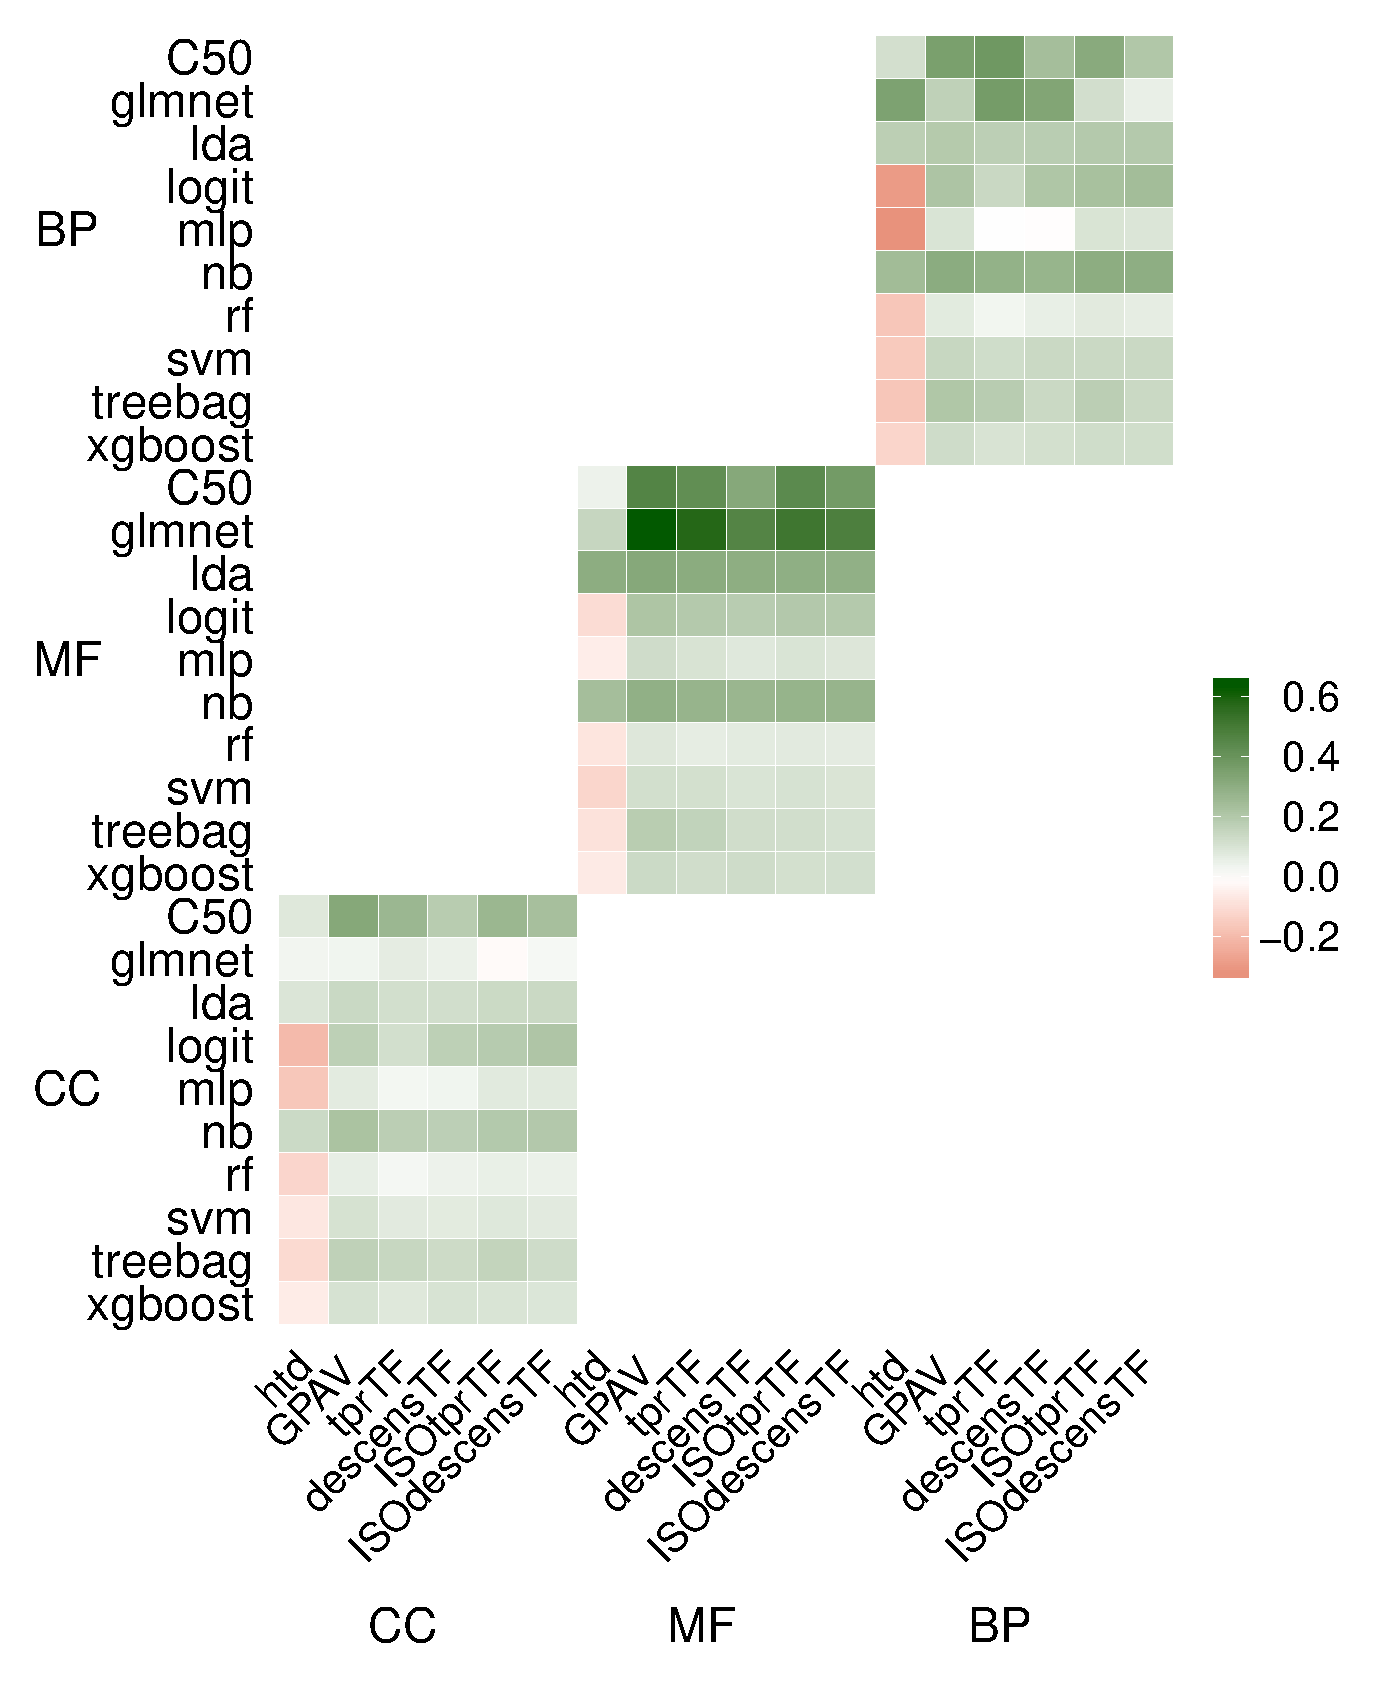
\includegraphics[scale=0.22]{./img/HEATMAP1.eps}
\end{figure}
\end{tframe}

\begin{tframe}{Confronto tra metodi ensemble}
\only<1>{
\highlightbf{AUPRC (arancio) AUROC(Blu) FS (36 punti = 12 algo * 3 onto)}
\begin{figure}
\centering
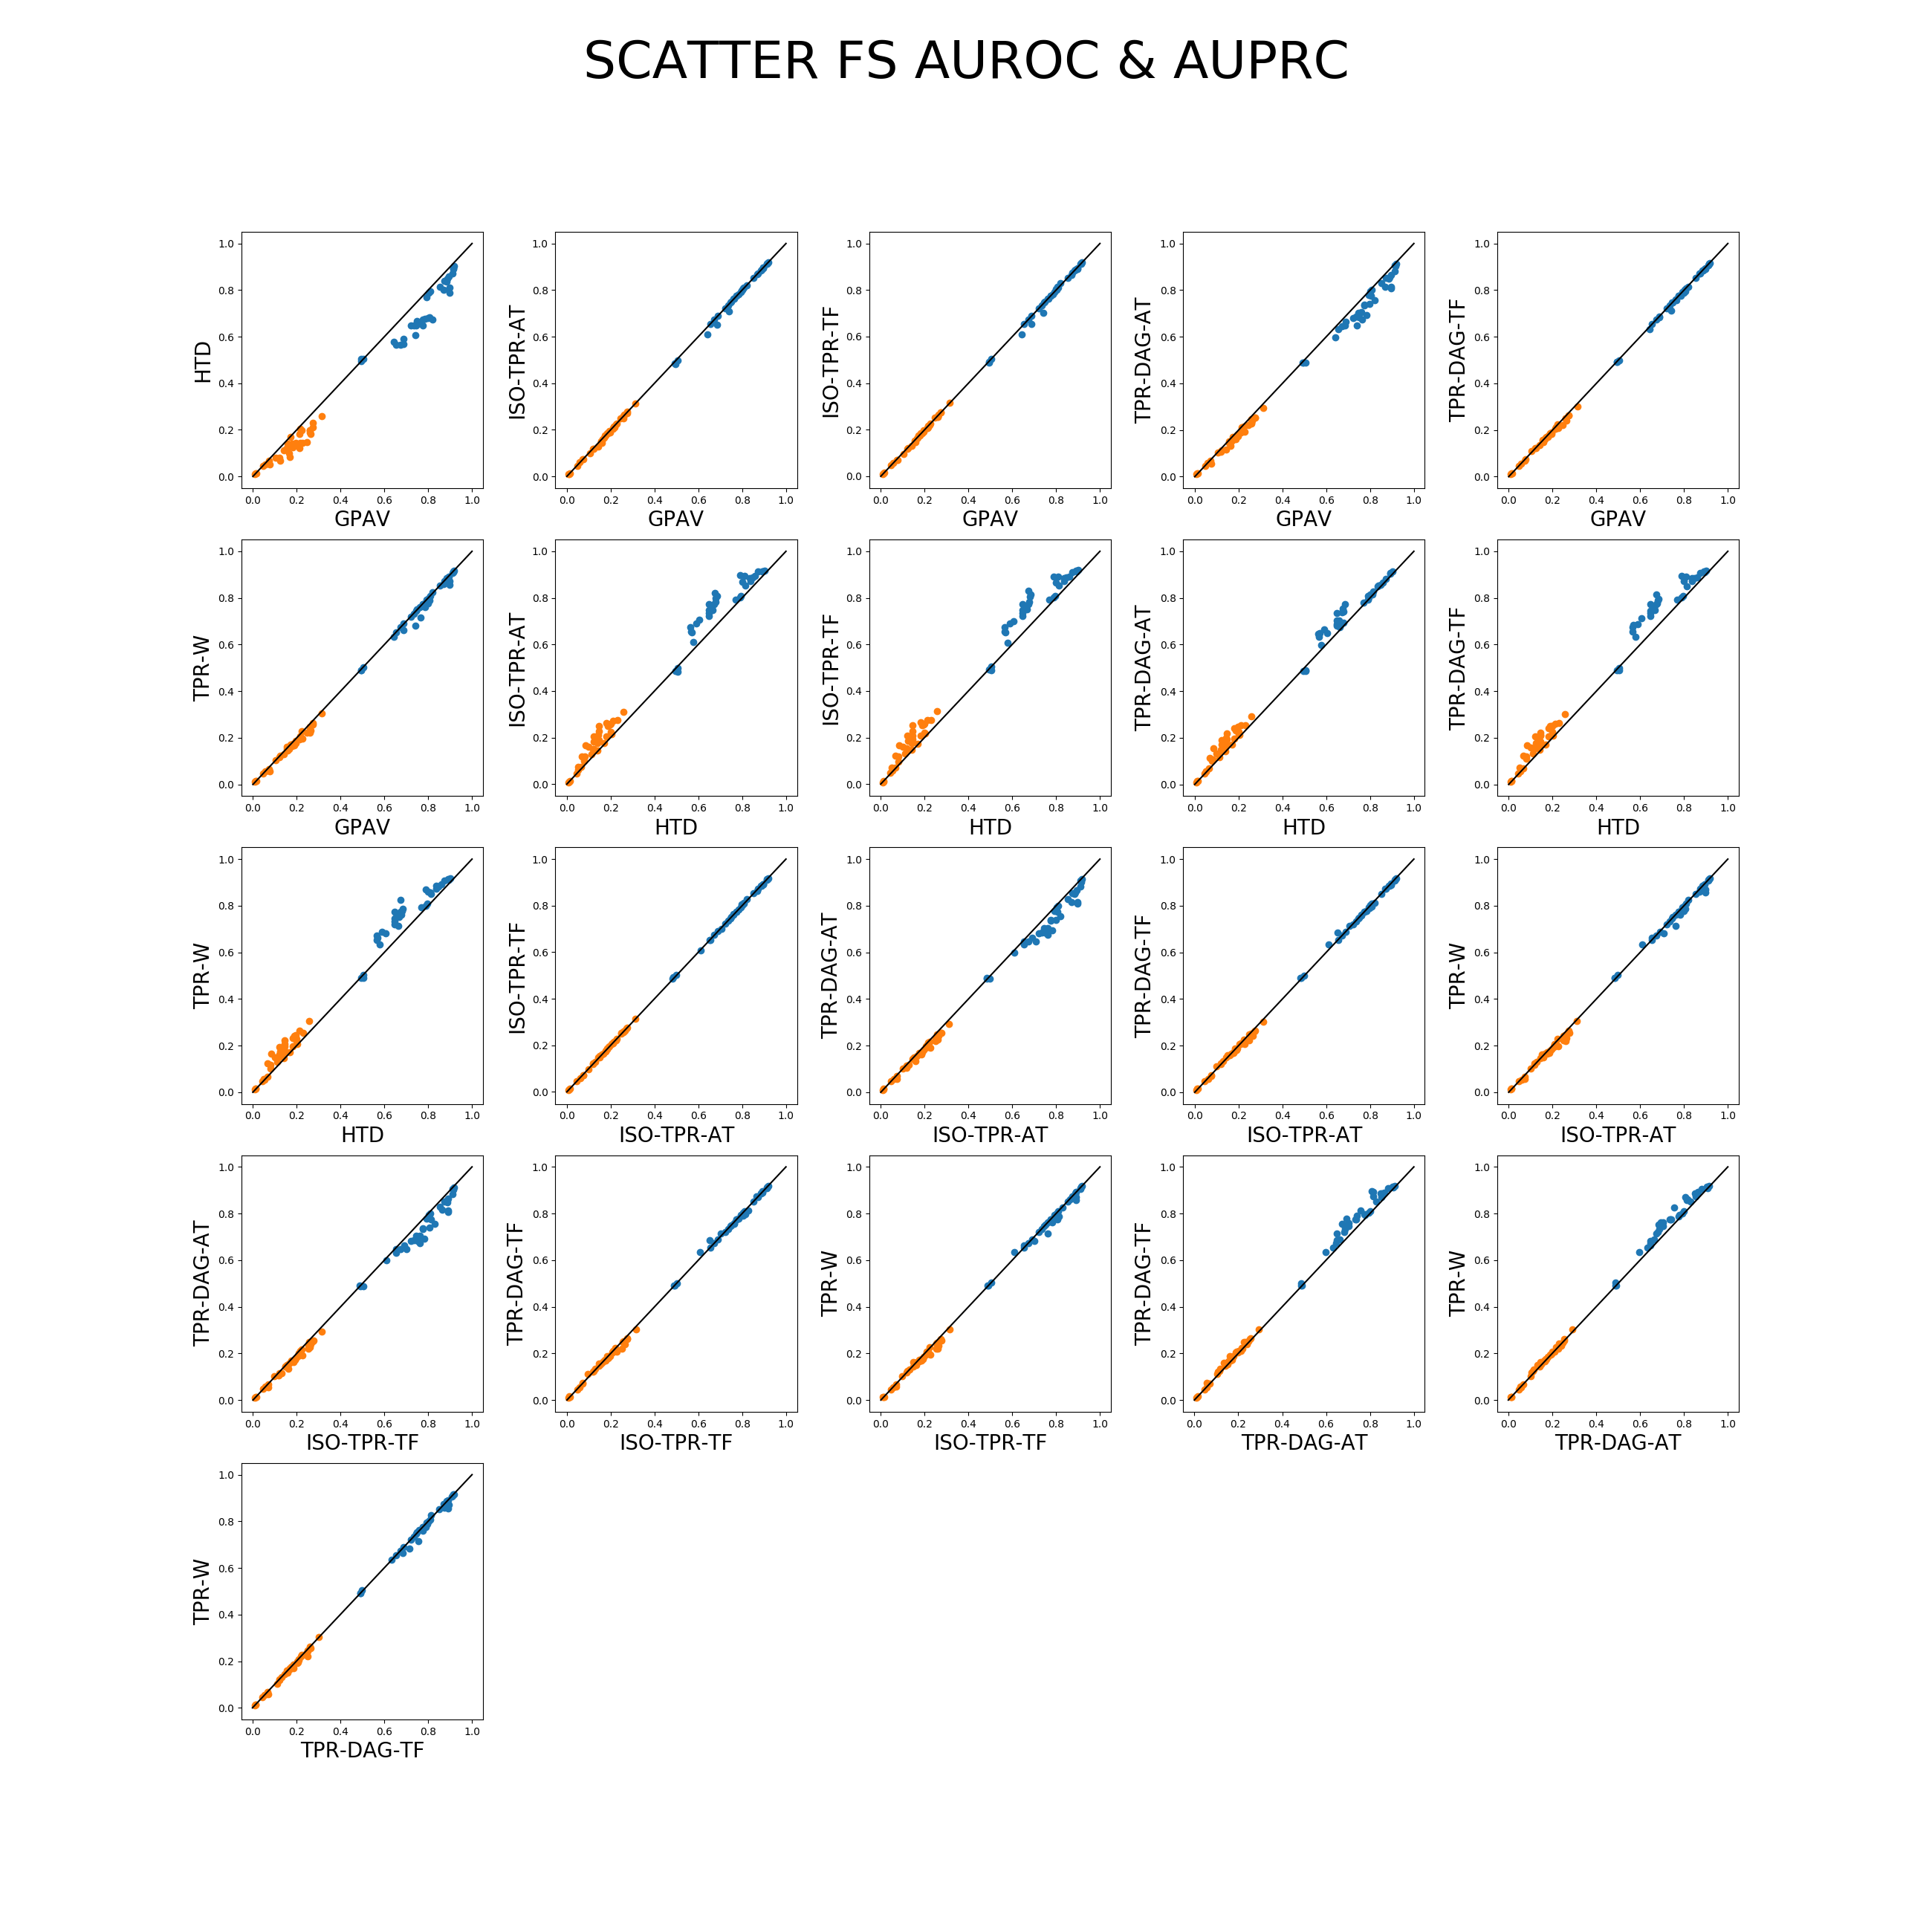
\includegraphics[scale=0.1]{../images/scatterplot_FS.png}
\end{figure}
}
\only<2>{
\highlightbf{AUPRC (arancio) AUROC(Blu) PCA (36 punti = 12 algo * 3 onto)}
\begin{figure}
\centering
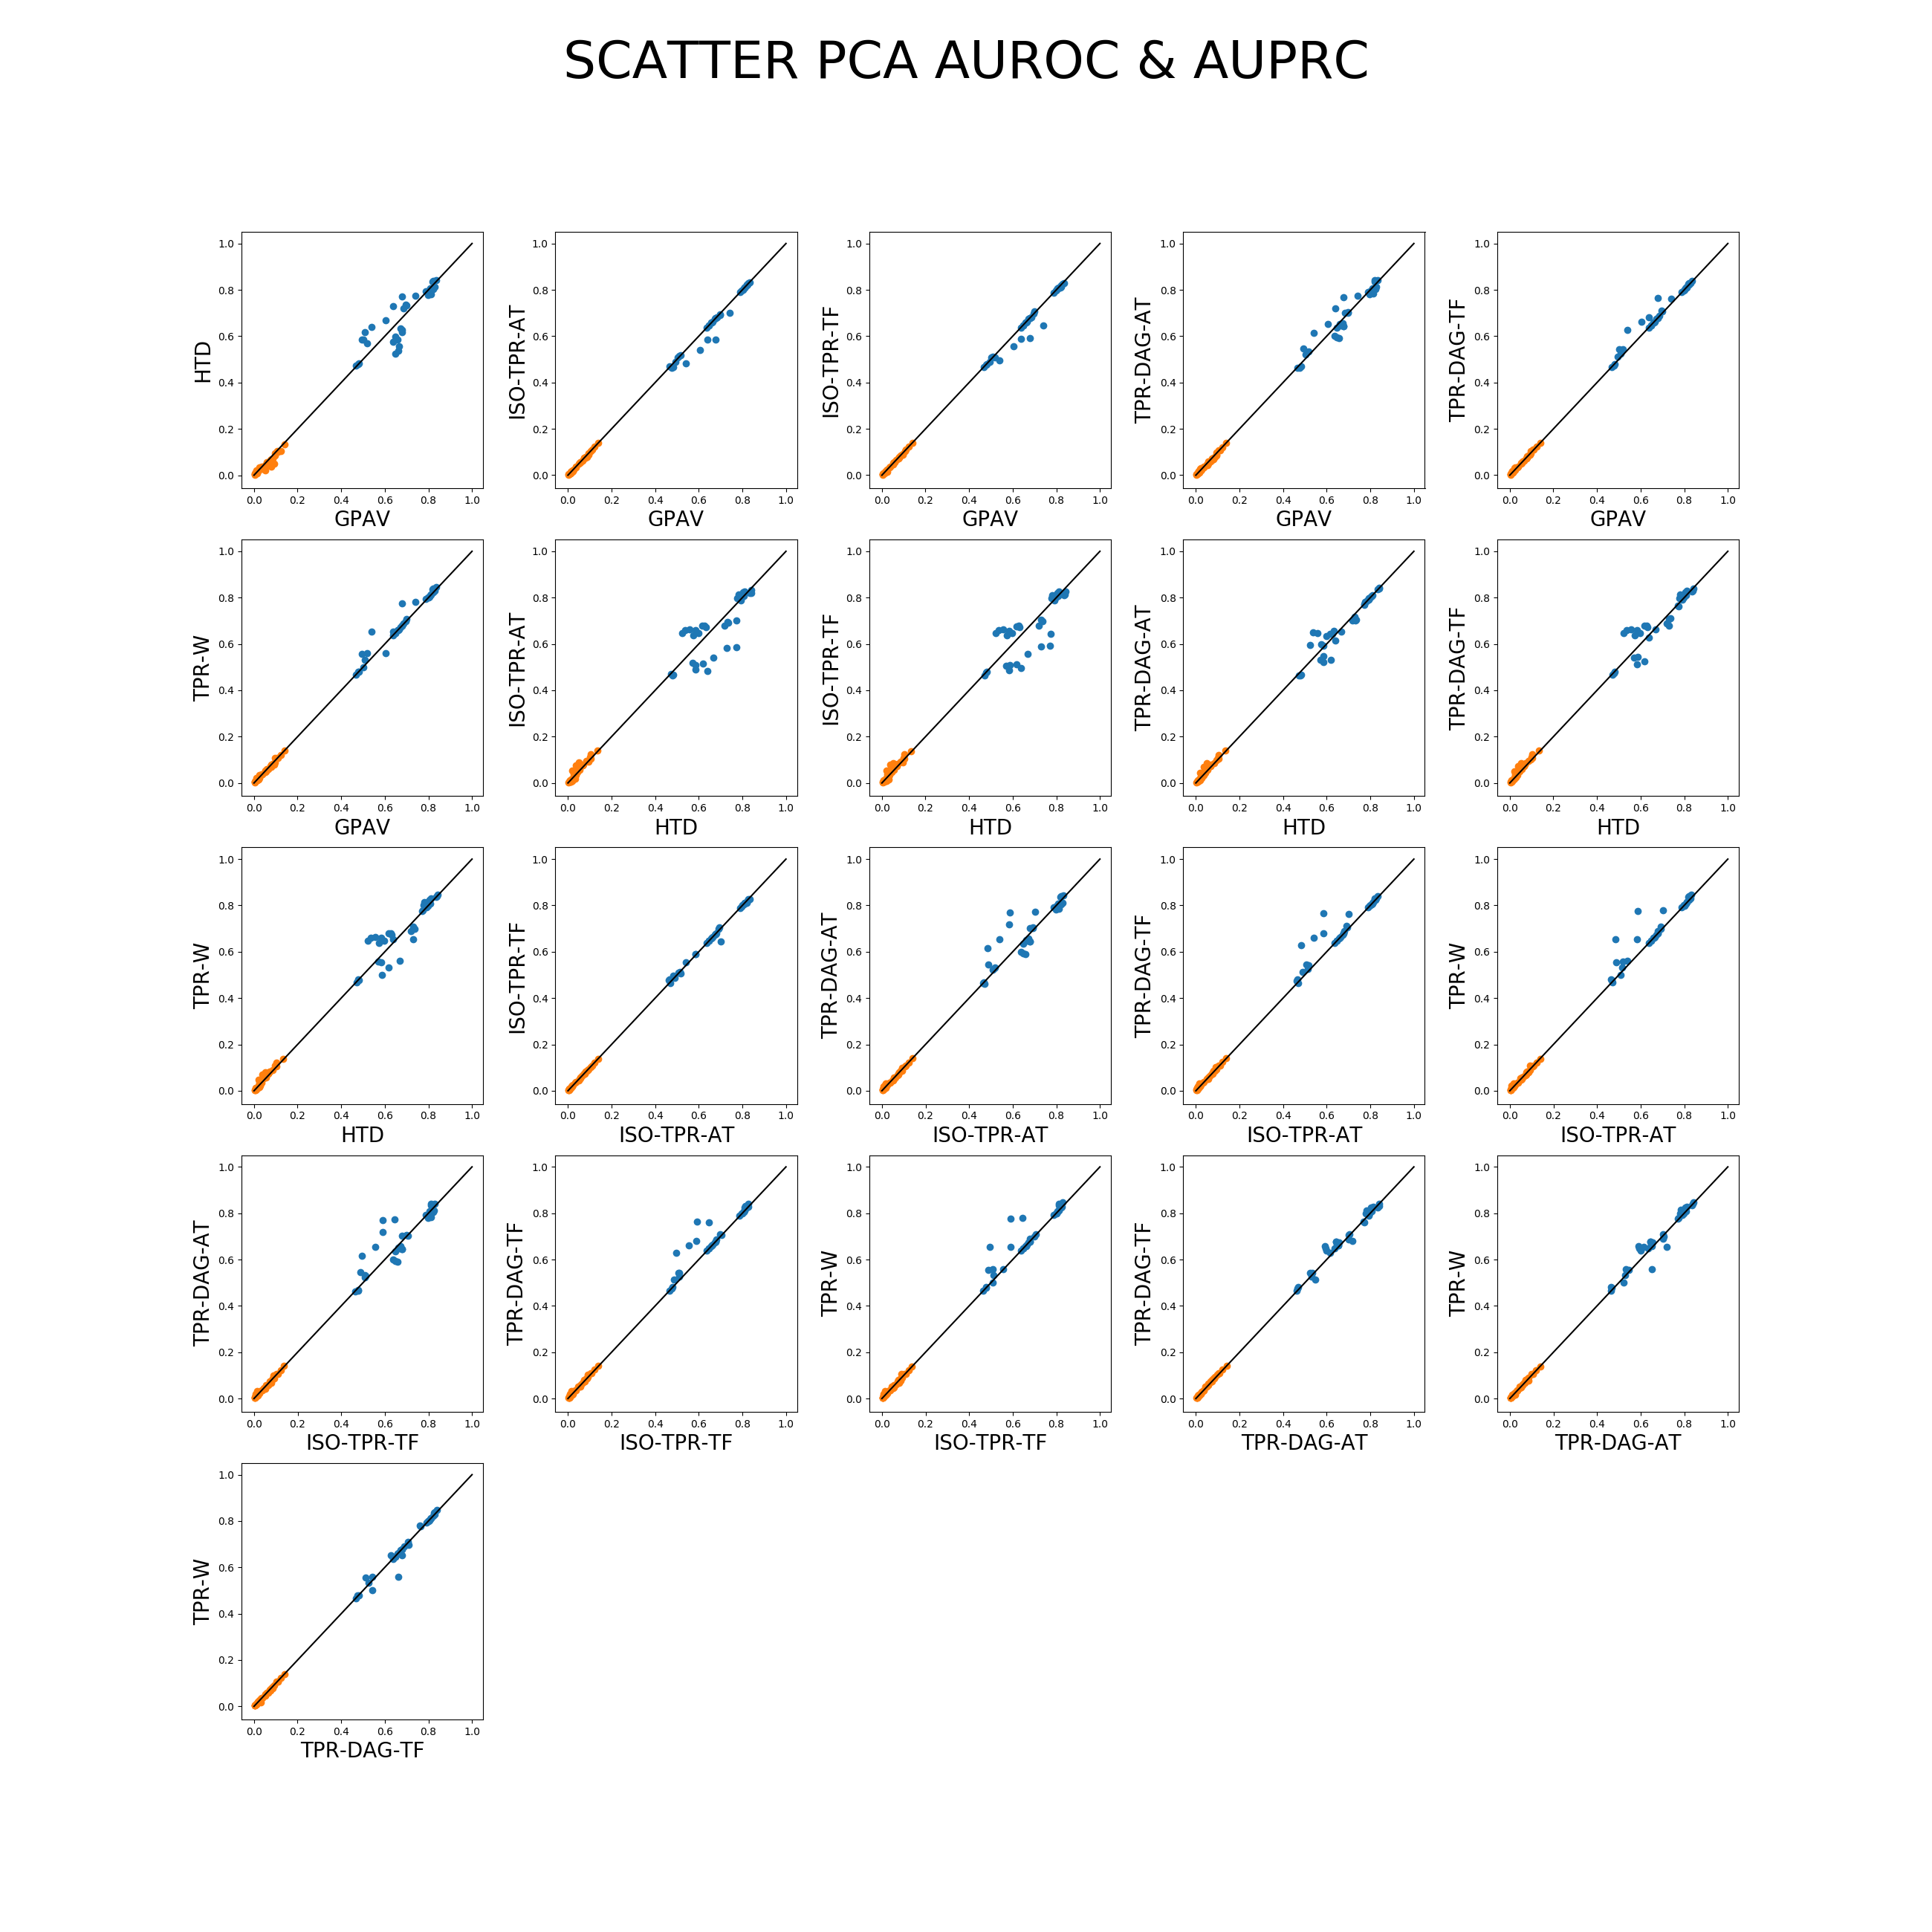
\includegraphics[scale=0.1]{../images/scatterplot_PCA.png}
\end{figure}
}
\end{tframe}
\begin{tframe}{Conclusioni}
\begin{itemize}
\onslide<1->
\item I metodi ensemble gerarchici riescono ad apportare miglioramenti statisticamente significativi alle performance dei predittori flat a patto di avere delle predizioni di partenza sufficientemente accurate.
\onslide<2->
\item La FS con correlazione di Pearson richiede tempi più lunghi della selezione con PCA, ma determina un vantaggio statisticamente significativo a livello di performance rispetto a quest’ultima (sia flat che ensemble).
\onslide<3->
\item Il tuning degli algoritmi flat svolge un ruolo importante. Alcuni algoritmi hanno prodotto predittori flat scadenti, che non hanno consentito ai metodi di ensemble gerarchici di migliorare le performance (es. i modelli lineari generalizzati, addestrati con il package glmnet in R).
\onslide<4->
\item I nuovi metodi ensemble gerarchici introdotti in questa tesi (GPAV e ISO-TPR), si sono dimostrati competitivi rispetto ai metodi ensemble gerarchici allo stato dell’arte, e in alcuni casi hanno prodotto risultati significativamente migliori rispetto ad algoritmi gerarchici allo stato dell'arte.
\end{itemize}
\end{tframe}
\begin{tframe}{Lavori futuri}
\begin{itemize}
\onslide<1->
\item Ampliare il numero di specie su cui effettuare l’analisi.
\onslide<2->
\item Effettuare un tuning più accurato degli algoritmi di machine learning selezionati, tenendo in considerazione che le classi dell’output strutturato sono
spesso sbilanciate all’interno dei dataset per la GO.
\onslide<3->
\item Introdurre nuove tecniche di riduzione della dimensionalità, sia per ridurre i tempi di calcolo (complessità) che per migliorare i risultati dei classificatori base (performance).
\onslide<4->
\item Utilizzare altre tipologie di selezione dei figli per lo step bottom-up della True Path Rule, in combinazione e non (a esempio effettuando una selezione
dei figli pesata con soglia adattiva).
\onslide<5->
\item Analizzare in maniera più approfondita le performance, ad esempio in relazione ad altre metriche, come la F-score gerarchica.
\onslide<6->
\item Confrontare i metodi ensemble con i diversi metodi per la predizione su
output strutturati, come ad esempio i metodi Kernel con output strutturato.
\end{itemize}
\end{tframe}
\begin{frame}{}
  \centering \Large
  \emph{\highlight{Grazie!}\\Domande?}
\end{frame}
\begin{tframe}{Bibliografia}
\begin{itemize}
\footnotesize{
\item G. Valentini,\emph{ Hierarchical Ensemble Methods for Protein Function Prediction}, ISRN Bioinformatics, 2014.
\item G. Valentini, \emph{True path rule hierarchical ensembles for genome-wide gene function prediction}, IEEE/ACM Transactions on Computational Biology and Bioinformatics, vol.8, no. 3, pp. 832–847, 2011.
\item N. Cesa-Bianchi, M. Re, G. Valentini, \emph{Synergy of multi-label hierarchical ensembles, data fusion, and cost-sensitive methods for gene functional inference}, Machine Learning, vol.88(1), pp. 209-241, 2012.
\item M. Notaro, M. Schubach, P. N. Robinson e Giorgio Valentini, \emph{Prediction of Human Phenotype Ontology terms by means of hierarchical ensemble methods}, BMC Bioinformatics, vol 18, numero 1, pagine 449, 12 Ottobre, 2017.
\item Burdakov O., Sysoev O., Grimvall A., Hussian M. \emph{An O(n2) Algorithm for Isotonic Regression.}, Large-Scale Nonlinear Optimization. Nonconvex Optimization and Its Applications, vol 83. Springer, 2006.
\item Szklarczyk D, Franceschini A, Wyder S, \emph{STRING v10: protein–protein interaction networks}, integrated over the tree of life, Nucleic Acids Research, 2015.}
\end{itemize}
\end{tframe}
\end{document}
